\documentclass[11pt]{article}

\usepackage[margin=1in]{geometry}
\usepackage{amsmath}
\usepackage{array}
\usepackage{booktabs}
\usepackage{caption}
\usepackage{float}
\usepackage{graphicx}
\usepackage{hyperref}
\usepackage{longtable}
\usepackage[numbers,sort&compress]{natbib}
\usepackage{setspace}

\graphicspath{{paper_assets_20260318T003344Z/figures/}}
\captionsetup{font=small}
\setstretch{1.08}
\hypersetup{colorlinks=true,citecolor=blue,linkcolor=blue,urlcolor=blue}

\title{Operational Weekly Dengue Forecasting in Bangladesh Using Hierarchy-Aware Panel Backtesting: Strong Baselines Remain Hard to Beat}
\author{Author names and affiliations to be added}
\date{\today}

\begin{document}
\maketitle

\begin{abstract}
\textbf{Background:} Dengue remains a growing public health threat globally and in Bangladesh, where recent outbreaks have been large, geographically widespread, and operationally demanding for the health system \citep{bhatt2013global,zheng2025global,hossain2023twentytwo,who2023bangladesh}. Yet much of the dengue forecasting literature still relies on climate-dominant predictor sets, limited validation, or retrospective study designs that do not map cleanly onto operational forecasting \citep{leung2023systematic}.

\textbf{Methods:} We framed the problem as weekly multi-geography forecasting of dengue case counts in Bangladesh and built a hierarchy-aware panel pipeline over 9 geographic series from 2021-12-27 to 2025-09-15. We repaired an overlapping Dhaka hierarchy by replacing \texttt{DHA\_DIV} with \texttt{DHA\_DIV\_OUT\_METRO}, then evaluated two tracks using direct multi-horizon rolling-origin backtesting: an operational 1--4 week track using case-history and calendar predictors only, and an experimental 5--12 week track that additionally used lagged climate features. Macro-averaged mean absolute error (MAE) across geography and horizon was the primary model-selection criterion.

\textbf{Findings:} Exploratory diagnostics showed a difficult but highly structured forecasting problem: zero proportions ranged from 3.1\% to 55.9\%, variance-to-mean ratios ranged from 61.4 to 2797.1, lag-1 autocorrelation ranged from 0.953 to 0.980, and lag-52 autocorrelation was weak to modest. Although all raw series satisfied a combined ADF/KPSS stationarity screen, rolling moments still showed outbreak-driven heteroskedasticity. In the operational track, persistence was the best overall model (MAE 154.218; RMSE 206.390), ahead of residual random forest (MAE 179.371), global Tweedie (MAE 181.767), residual histogram gradient boosting (MAE 183.082), panel histogram gradient boosting (MAE 296.576), and seasonal naive forecasting (MAE 520.177). Persistence also remained the strongest experimental model at horizons 5--12. Climate-augmented models did not outperform persistence in the current data window.

\textbf{Interpretation:} Under realistic hierarchy constraints, small-sample weekly surveillance data, major outbreak regime shifts, and incomplete real-time weather coverage, strong autoregressive baselines remain difficult to beat for operational dengue forecasting in Bangladesh. The clearest near-term path is therefore not immediate escalation to more complex architectures, but better regime-aware residual correction, geography-specific error analysis, and improved covariate timeliness.
\end{abstract}

\section{Introduction}
Dengue is one of the most important mosquito-borne viral diseases globally, with burden increasing over recent decades and substantial morbidity concentrated in tropical and subtropical settings \citep{bhatt2013global,zheng2025global}. In Bangladesh, dengue has shifted from an episodic concern to a recurrent national public health threat, with increasingly large outbreaks, expanding geographic spread, and growing pressure on hospital services \citep{hossain2023twentytwo}. The 2023 outbreak made the operational challenge especially clear: by 7 August 2023, Bangladesh had already reported 69,483 laboratory-confirmed cases and 327 deaths, with transmission no longer confined to Dhaka and cases accelerating earlier than in typical seasonal surges \citep{who2023bangladesh}.

Accurate short-horizon forecasting could support hospital preparedness, situational awareness, and resource allocation. However, dengue forecasting is difficult in practice because the signal is shaped by short-run epidemic momentum, strong spatial heterogeneity, intermittent zeros in lower-burden locations, imperfect seasonality, and often incomplete exogenous data. A recent systematic review of 99 dengue prediction models found heavy reliance on climate predictors, limited external validation, and inconsistent reporting of modeling choices and performance \citep{leung2023systematic}. These shortcomings are especially problematic when the end goal is operational forecasting rather than retrospective fit.

Existing forecasting studies in Bangladesh have been useful but still leave an operational gap. Prior work has included national ARIMA-style forecasting and division-level monthly machine learning comparisons \citep{naher2022forecasting,liu2025comparative}. Those studies contributed important early evidence, but they were not designed around weekly geographically disaggregated panel forecasting with hierarchy repair, direct multi-horizon training, and rolling-origin validation focused on operational deployment. More broadly, epidemic forecasting evaluations show that model ranking is horizon-dependent, unstable across validation windows, and highly sensitive to the choice of baseline and scoring design \citep{cramer2022evaluation}.

This study addresses that gap. Rather than asking which sophisticated model appears most flexible in principle, we ask a more operational question: given the currently available weekly dengue and climate data in Bangladesh, what forecasting design is most trustworthy for 1--4 week deployment, and what does a robust benchmarking exercise actually reveal? The answer is important whether the result is positive or negative. If complex models provide stable gains, that supports escalation. If they do not, that is still actionable evidence for surveillance operations and for the next round of model development.

\section{Related Work and Study Contribution}
Three strands of prior work shaped this study. First, dengue forecasting reviews emphasize that many published models rely heavily on climate data, under-document validation procedures, and rarely demonstrate robust real-world generalization \citep{leung2023systematic}. Second, Bangladesh-specific studies have shown that both time-series and machine learning approaches can capture some dengue dynamics, especially at monthly resolution \citep{naher2022forecasting,liu2025comparative}. Third, hierarchical forecasting and outbreak-forecast evaluation research show that forecast design, aggregation logic, and validation strategy matter as much as model class \citep{hyndman2011optimal,hyndman2021forecasting,cramer2022evaluation}.

Against that backdrop, our study makes four concrete contributions.
\begin{enumerate}
    \item It defines the forecasting task explicitly as weekly, multi-geography, multi-horizon count forecasting, with macro-averaged MAE across geography and horizon as the primary model-selection criterion.
    \item It repairs an overlapping Dhaka geography so that bottom-level modeling and country-level roll-up are coherent.
    \item It separates modeling into two tracks: an operational track that reflects realistic deployment constraints and an experimental track that tests whether weather adds value at longer horizons.
    \item It shows, using rolling-origin backtesting, that persistence remains the strongest operational model overall despite several reasonable challenger families.
\end{enumerate}

That final result is scientifically useful. In applied forecasting, especially in public health, a well-demonstrated negative result can be more informative than a weakly supported positive one. If robust baselines remain dominant after careful diagnostics and backtesting, then the empirical message is that the current data-generating environment rewards simplicity, recency, and stability.

\section{Data and Forecasting Task}
\subsection{Data Sources}
Weekly dengue case counts were assembled from Bangladesh surveillance data released through the Directorate General of Health Services. Environmental covariates were aggregated as weekly polygon-area-weighted climate features from the pipeline's configured ERA5/IMERG source. The final case panel covered 2021-12-27 to 2025-09-15, while climate covariates extended from 2021-12-20 to 2025-06-30, leaving an 11-week gap between the latest climate week and the latest case week.

The raw case data contained 195 weekly observations per geographic series and no missing weeks at the weekly panel level. The modeling geography initially included an overlap in which \texttt{DHA\_DIV} contained \texttt{DHA\_METRO}. Because overlapping bottom-level nodes invalidate coherent aggregation, we replaced \texttt{DHA\_DIV} with \texttt{DHA\_DIV\_OUT\_METRO} before modeling. The resulting hierarchy repair had zero closure error.

\subsection{Forecasting Task Definition}
We defined the target as weekly dengue case counts at the \texttt{geo\_id} level on the original count scale. The operational task was 1--4 week forecasting. A secondary experimental task covered 5--12 week forecasting. Forecasts were generated for each geography and horizon, and then evaluated per geography and per horizon before macro-averaging. This choice prevented Dhaka-dominant volumes from masking poor performance in lower-burden regions.

\begin{table}[H]
\centering
\small
\caption{Study design summary.}
\label{tab:study-design}
\begin{tabular}{@{}p{0.34\textwidth}p{0.56\textwidth}@{}}
\toprule
Item & Value \\
\midrule
Forecast target & Weekly dengue case counts \\
Temporal grain & Weekly \\
Spatial grain & \texttt{geo\_id} \\
Operational horizon & 1 to 4 weeks ahead \\
Experimental horizon & 5 to 12 weeks ahead \\
Primary KPI & Macro-averaged MAE across geography and horizon \\
Secondary KPI & Macro-averaged RMSE \\
Forecast strategy & Direct multi-horizon, not recursive \\
Operational covariates & Case-history and calendar features only \\
Experimental covariates & Case-history, calendar, and climate features \\
Hierarchy repair & \texttt{DHA\_DIV} replaced by \texttt{DHA\_DIV\_OUT\_METRO} \\
\bottomrule
\end{tabular}
\end{table}

\section{Exploratory Diagnostics}
We conducted a deliberately broad set of diagnostics before model training: missing-week checks, ADF and KPSS stationarity tests, STL decomposition, autocorrelation analysis, rolling moments, zero-inflation summaries, overdispersion checks, cross-geography correlation, hierarchy consistency checks, and climate lead-lag analysis. This diagnostic pass served two purposes. First, it informed model specification. Second, it created an interpretable empirical record for the paper rather than treating EDA as a disposable preprocessing step.

The geography-level series were extremely heterogeneous. After hierarchy repair, mean weekly cases ranged from 10.1 in Sylhet to 1003.5 in Dhaka Metro. Zero-week proportions ranged from 3.1\% in Dhaka Metro to 55.9\% in Sylhet. Variance-to-mean ratios ranged from 61.4 to 2797.1, indicating severe overdispersion across all series. Short-run dependence was strong everywhere: lag-1 autocorrelation ranged from 0.953 to 0.980. By contrast, lag-52 autocorrelation ranged from $-0.078$ to 0.219, indicating that annual repetition existed but was far weaker than immediate autoregressive persistence.

The stationarity screen needs nuance. All nine raw series passed a combined ADF/KPSS rule as stationarity candidates, eight of nine \texttt{log1p}-transformed series also passed, and all nine first-differenced series passed. Formally, that means the data do not behave like textbook unit-root series. Practically, however, rolling means and rolling standard deviations changed sharply through outbreak periods, especially during the 2023 wave. We therefore treated the series as highly persistent, outbreak-driven, and heteroskedastic rather than assuming a simple weak-stationarity regime.

Seasonality was present but not strong enough to dominate the task. Geography-specific peak weeks clustered broadly in the late monsoon and post-monsoon period, while STL decomposition showed seasonal structure of modest strength. Yet the seasonal naive benchmark underperformed severely in the backtests. This was an important negative finding in the EDA stage itself: the data contain seasonal patterning, but the operational problem is governed much more strongly by recent case momentum than by clean annual repetition.

Finally, the climate diagnostics were informative but operationally constrained. Dew point, temperature, humidity, rain, and soil moisture showed plausible lead-lag relationships with future cases, often at multiweek lags. However, because climate coverage ended 11 weeks before the latest case week, any operational model that required contemporaneous weather would fail or require imputation precisely where real-time deployment matters most. That observation motivated the separation between operational and experimental modeling tracks.

\section{Methods}
\subsection{Forecasting Strategy}
The forecasting system used a direct multi-horizon strategy rather than recursive forecasting \citep{hyndman2021forecasting}. Each horizon had its own prediction rule or trained model. Forecasts at horizon 1 were not fed into horizon 2, horizon 2 forecasts were not fed into horizon 3, and so forth. We chose this strategy because forecast error characteristics differed materially by horizon, and because horizon-specific training makes evaluation easier to interpret under regime shifts.

\subsection{Dependent Variables}
Two dependent-variable formulations were used. For direct case models, the response was the future case count,
\[
y_{t+h},
\]
where $t$ denotes the forecast origin and $h$ the forecast horizon. For residual-correction models, the response was
\[
y_{t+h} - y_t,
\]
that is, the deviation from the persistence baseline. Residual models therefore learned how future counts depart from the most recent observed weekly count.

\subsection{Independent Variables}
The operational track used only signals that were available in real time at the forecast origin:
\begin{itemize}
    \item current weekly cases,
    \item case lags at 1, 2, 3, 4, 8, 13, 26, and 52 weeks,
    \item rolling means over 2, 4, and 8 weeks,
    \item \texttt{log1p(cases)},
    \item calendar features including week-of-year, seasonal sine/cosine terms, and a monsoon indicator,
    \item geography identity as a categorical input in pooled global models.
\end{itemize}

The experimental track added lagged and rolled climate variables for rain, near-surface temperature, humidity, dew point, and soil moisture. We deliberately did not make weather a required operational input because of the 11-week climate coverage gap.

\subsection{Model Ladder}
The baseline and challenger sequence was chosen to answer an operational question, not merely to maximize model diversity. The ladder consisted of:
\begin{itemize}
    \item \textbf{Persistence:} future cases equal the latest observed cases.
    \item \textbf{Seasonal naive$_{52}$:} future cases equal the value observed 52 weeks earlier.
    \item \textbf{Global Tweedie autoregressive model:} a regularized count model using pooled multi-geography training.
    \item \textbf{Global histogram gradient boosting model:} a pooled nonlinear count model using lag and calendar features.
    \item \textbf{Residual histogram gradient boosting:} a persistence-anchored correction model.
    \item \textbf{Residual random forest:} another persistence-anchored correction model.
\end{itemize}

Deep learning models were not included in the primary operational ladder. With only 195 weekly observations per series and 9 geographic series overall, this dataset is small for high-capacity sequence models, making overfitting a more likely immediate outcome than stable operational gain. Those models remain candidates for later experimental work, but not for first-line operational promotion.

\subsection{Validation Design and Metrics}
We used five rolling-origin folds spanning both relatively calm windows and outbreak-heavy validation windows. Fold F4 was especially important because it isolates the second half of 2023, when the epidemic regime changed sharply. This design follows the logic of outbreak forecasting evaluation in which performance must be judged across multiple temporal contexts rather than on a single hold-out block \citep{cramer2022evaluation}.

The primary metric was macro-averaged MAE across geography and horizon. RMSE was the secondary metric. Metrics were computed per geography and per horizon, then averaged. Pooled totals were retained for descriptive use only and were not used as the primary model-selection rule.

\subsection{Operational Stability Guard}
We added a simple but important operational safeguard. For trainable models, predictions were checked against the scale of the training data. If a fitted model produced implausibly explosive forecasts relative to the observed training range, that fit was logged as unstable and the corresponding predictions were reverted to the persistence baseline. This design choice is less glamorous than unrestricted model fitting, but it is more consistent with a deployable forecasting system.

\section{Results}
\subsection{Operational Track: Overall Ranking}
Table~\ref{tab:operational-leaderboard} summarizes the main operational results. Persistence remained the best overall model, with macro-averaged MAE 154.218 and RMSE 206.390. The closest challenger was the residual random forest, followed by the global Tweedie model and the residual histogram gradient boosting model. Seasonal naive forecasting performed dramatically worse than all operational alternatives.

\begin{table}[H]
\centering
\caption{Operational validation leaderboard. Metrics are macro-averaged across geography and horizon.}
\label{tab:operational-leaderboard}
\begin{tabular}{lrr}
\toprule
Model & MAE & RMSE \\
\midrule
Persistence & 154.218 & 206.390 \\
Residual random forest & 179.371 & 234.354 \\
AR Tweedie global & 181.767 & 241.761 \\
Residual HistGBM & 183.082 & 249.362 \\
Panel HistGBM & 296.576 & 367.618 \\
Seasonal naive$_{52}$ & 520.177 & 714.417 \\
\bottomrule
\end{tabular}
\end{table}

\begin{figure}[H]
\centering
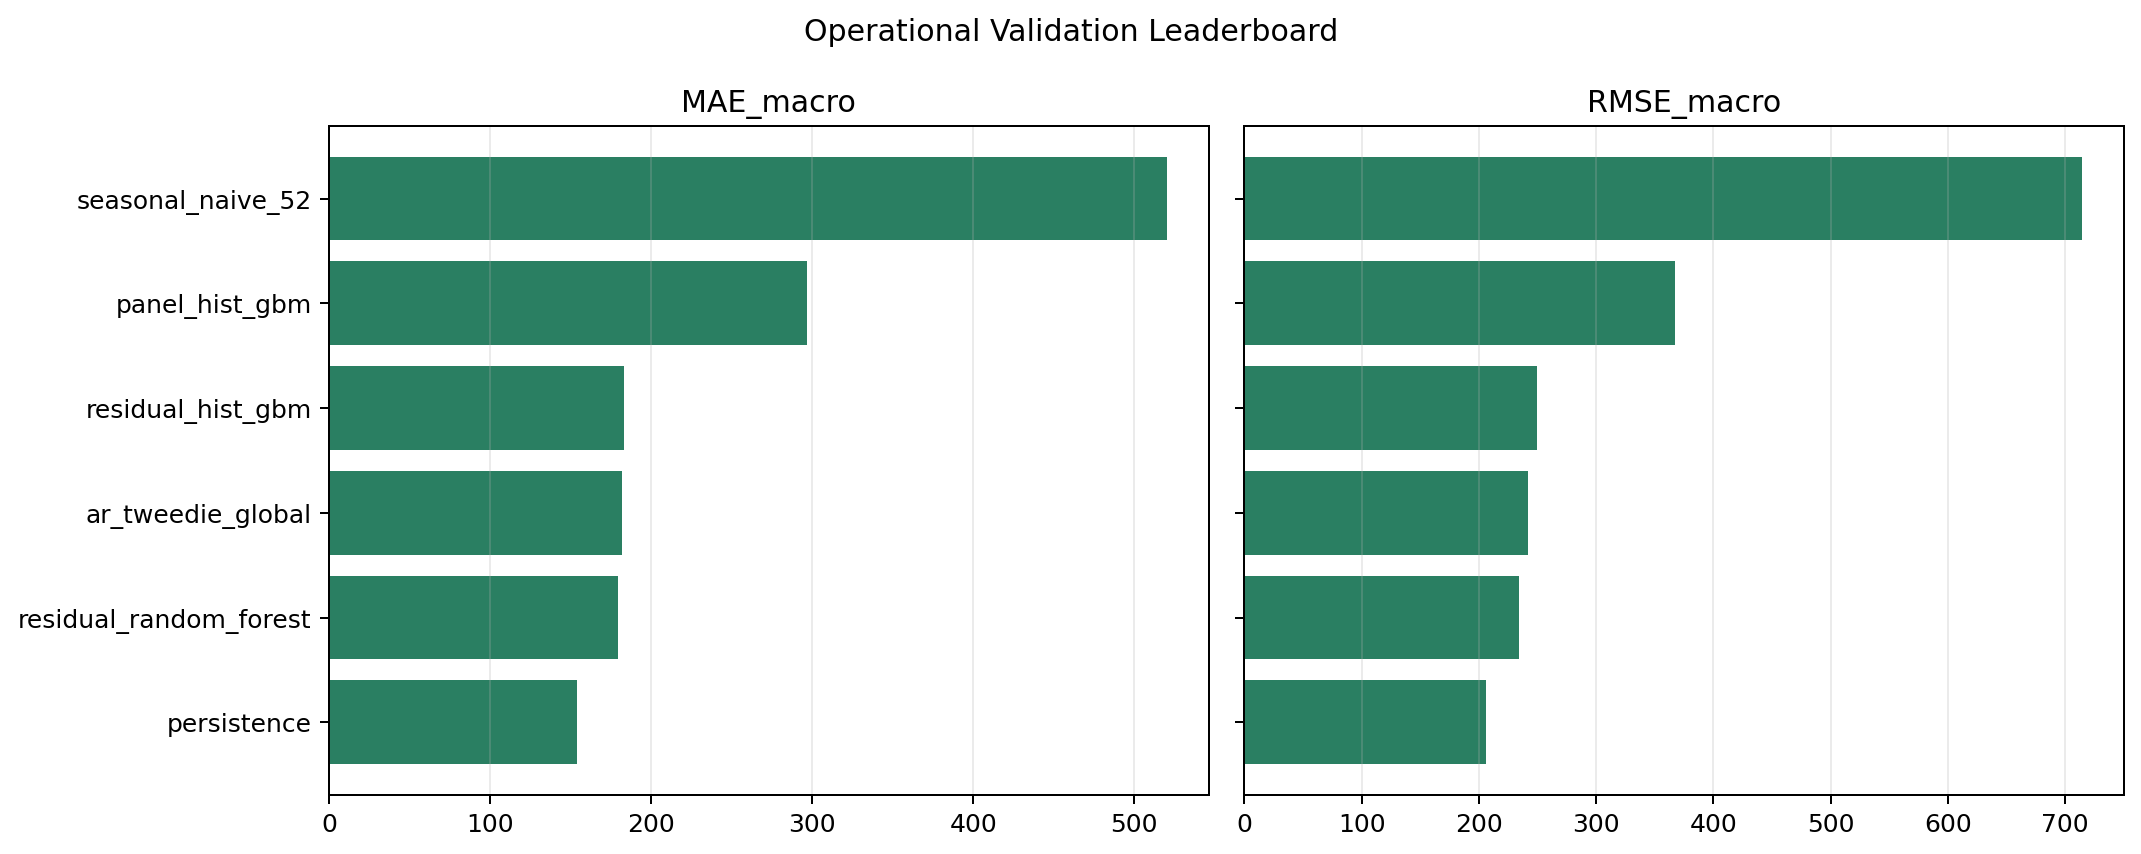
\includegraphics[width=0.92\textwidth]{fig_01_operational_leaderboard.png}
\caption{Operational validation leaderboard. Persistence remained the strongest overall operational model.}
\label{fig:operational-leaderboard}
\end{figure}

This result should not be misread as saying that all model-based challengers failed uniformly. Rather, no challenger provided consistent enough improvement across geographies, horizons, and folds to displace persistence as the operational default. In an operational setting, that distinction matters more than occasional fold wins.

\subsection{Horizon-Specific Performance}
Persistence was the best model at every operational horizon. Its macro-averaged MAE increased from 76.0 at horizon 1 to 227.3 at horizon 4, reflecting the expected degradation in short-term predictability as the lead time expands. This pattern is consistent with broader epidemic forecasting experience, where near-term accuracy decays with horizon even under strong models \citep{cramer2022evaluation}.

\begin{figure}[H]
\centering
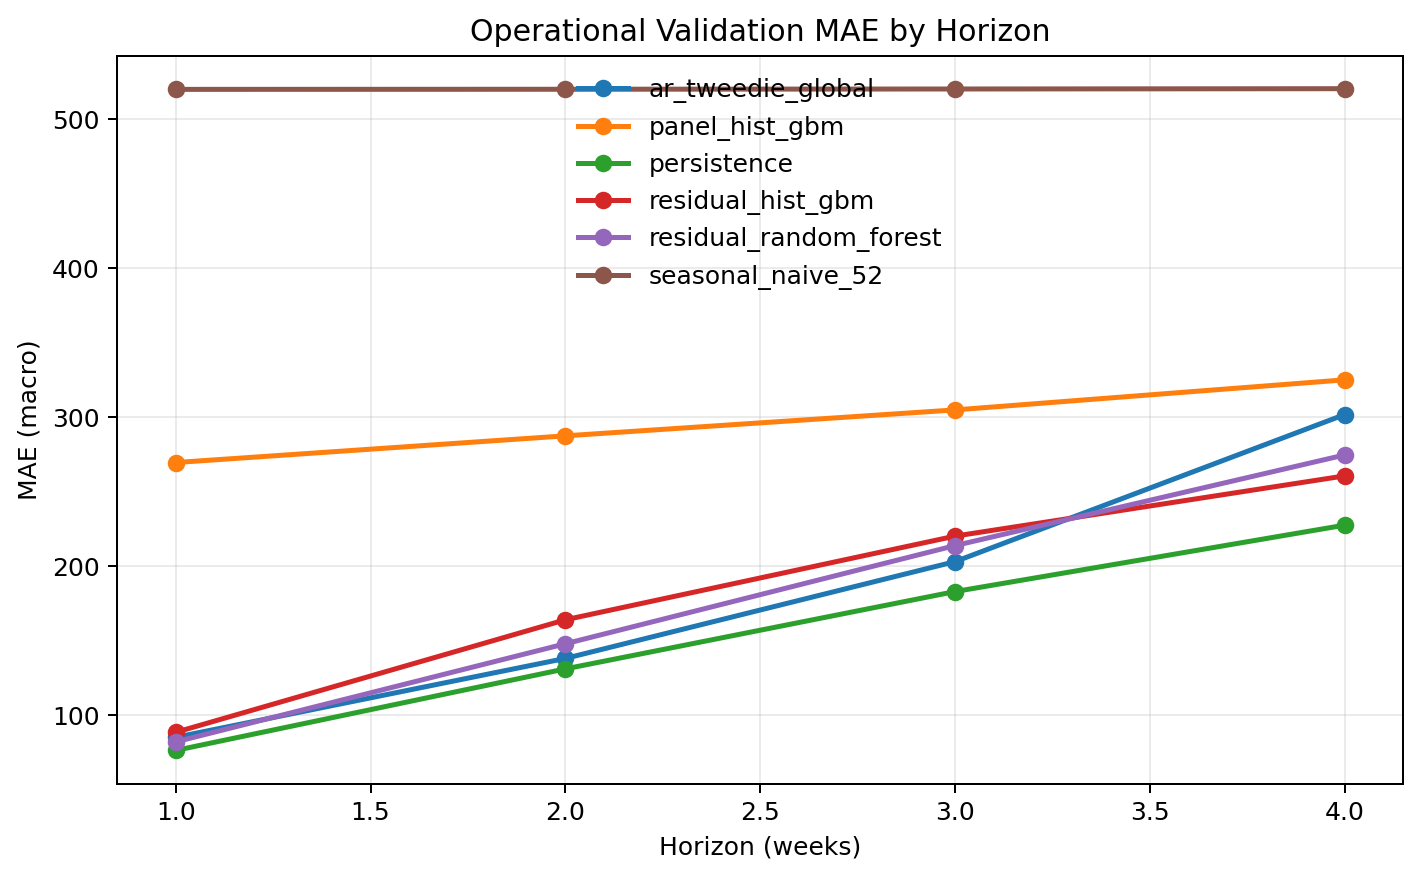
\includegraphics[width=0.82\textwidth]{fig_02_operational_horizon_mae.png}
\caption{Operational MAE by horizon. Persistence remains the best model from 1 to 4 weeks ahead, although all models degrade with lead time.}
\label{fig:operational-horizon}
\end{figure}

The horizon result is important because it rules out a common fallback interpretation, namely that complex models may still have been winning at the longest short-term horizons. They were not. Within the 1--4 week operational window, persistence remained the best performer at each horizon considered separately.

\subsection{Fold-Level and Geography-Level Heterogeneity}
The fold breakdown was more nuanced than the overall ranking. In folds F1, F2, and F5, the global histogram gradient boosting model achieved the lowest fold-level MAE. In fold F3, persistence performed best. In fold F4, which captures the second half of 2023 and therefore the major outbreak regime, the residual histogram gradient boosting model was the fold winner. Nevertheless, persistence remained the most stable model overall because it did not collapse catastrophically when the data-generating regime changed.

\begin{figure}[H]
\centering
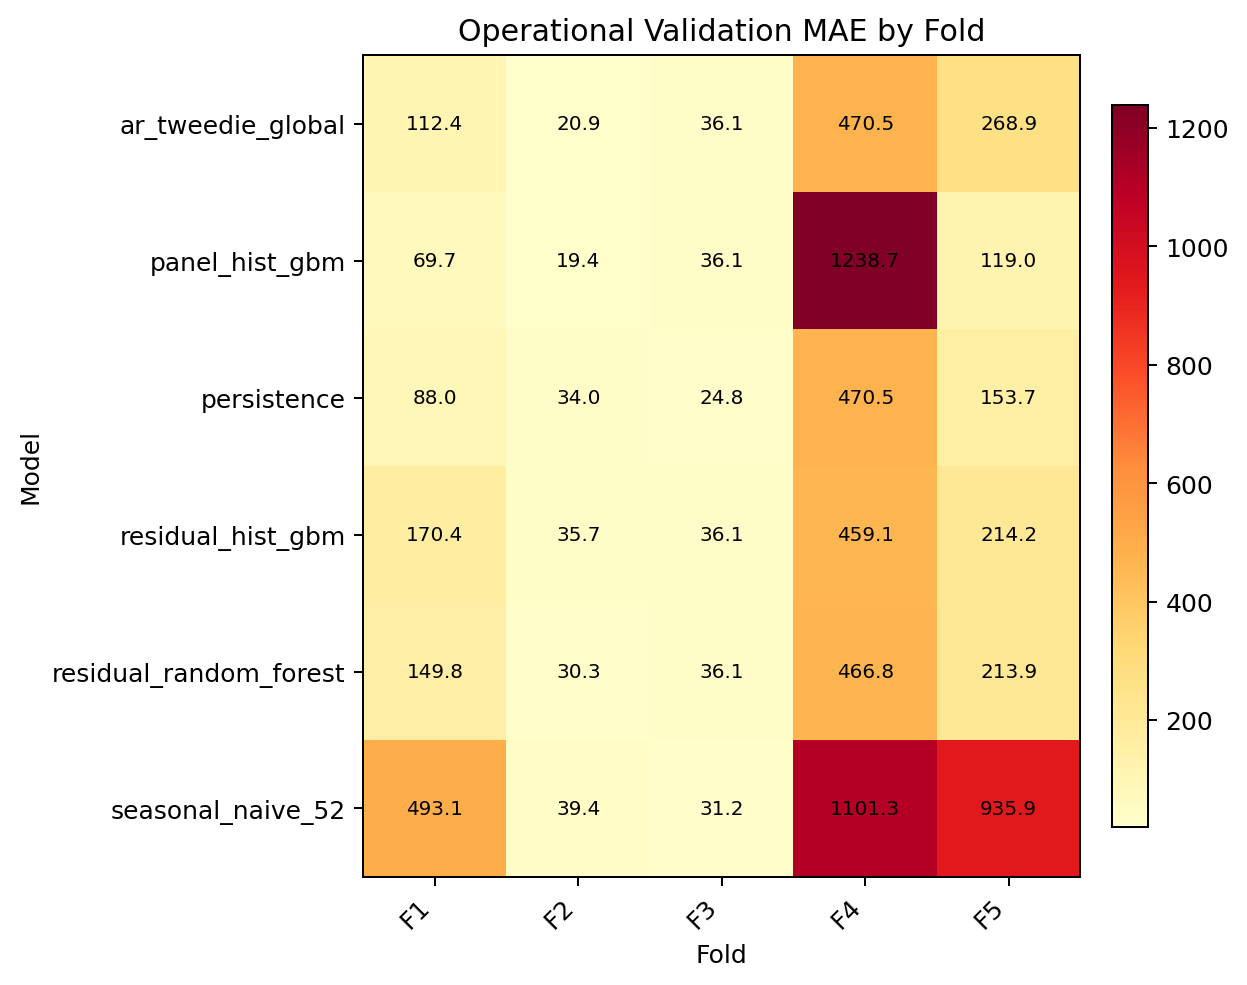
\includegraphics[width=0.72\textwidth]{fig_03_operational_fold_mae_heatmap.png}
\caption{Operational MAE by fold. Challenger models can win in specific windows, but their gains are not stable enough across folds to overtake persistence overall.}
\label{fig:operational-folds}
\end{figure}

Geography-level performance told a similarly informative story. Persistence was best in Barishal, Chattogram, Dhaka Metro, Khulna, and Sylhet. The Tweedie model marginally outperformed persistence in \texttt{DHA\_DIV\_OUT\_METRO}, Mymensingh, Rajshahi, and Rangpur. That pattern suggests that regularized count models may be especially promising in lower-volume or sparser regional series, even though they did not win the overall operational leaderboard. Interestingly, the residual random forest finished second overall without being the best model in any single geography, indicating broad but insufficient improvement over the pooled error surface.

\begin{figure}[H]
\centering
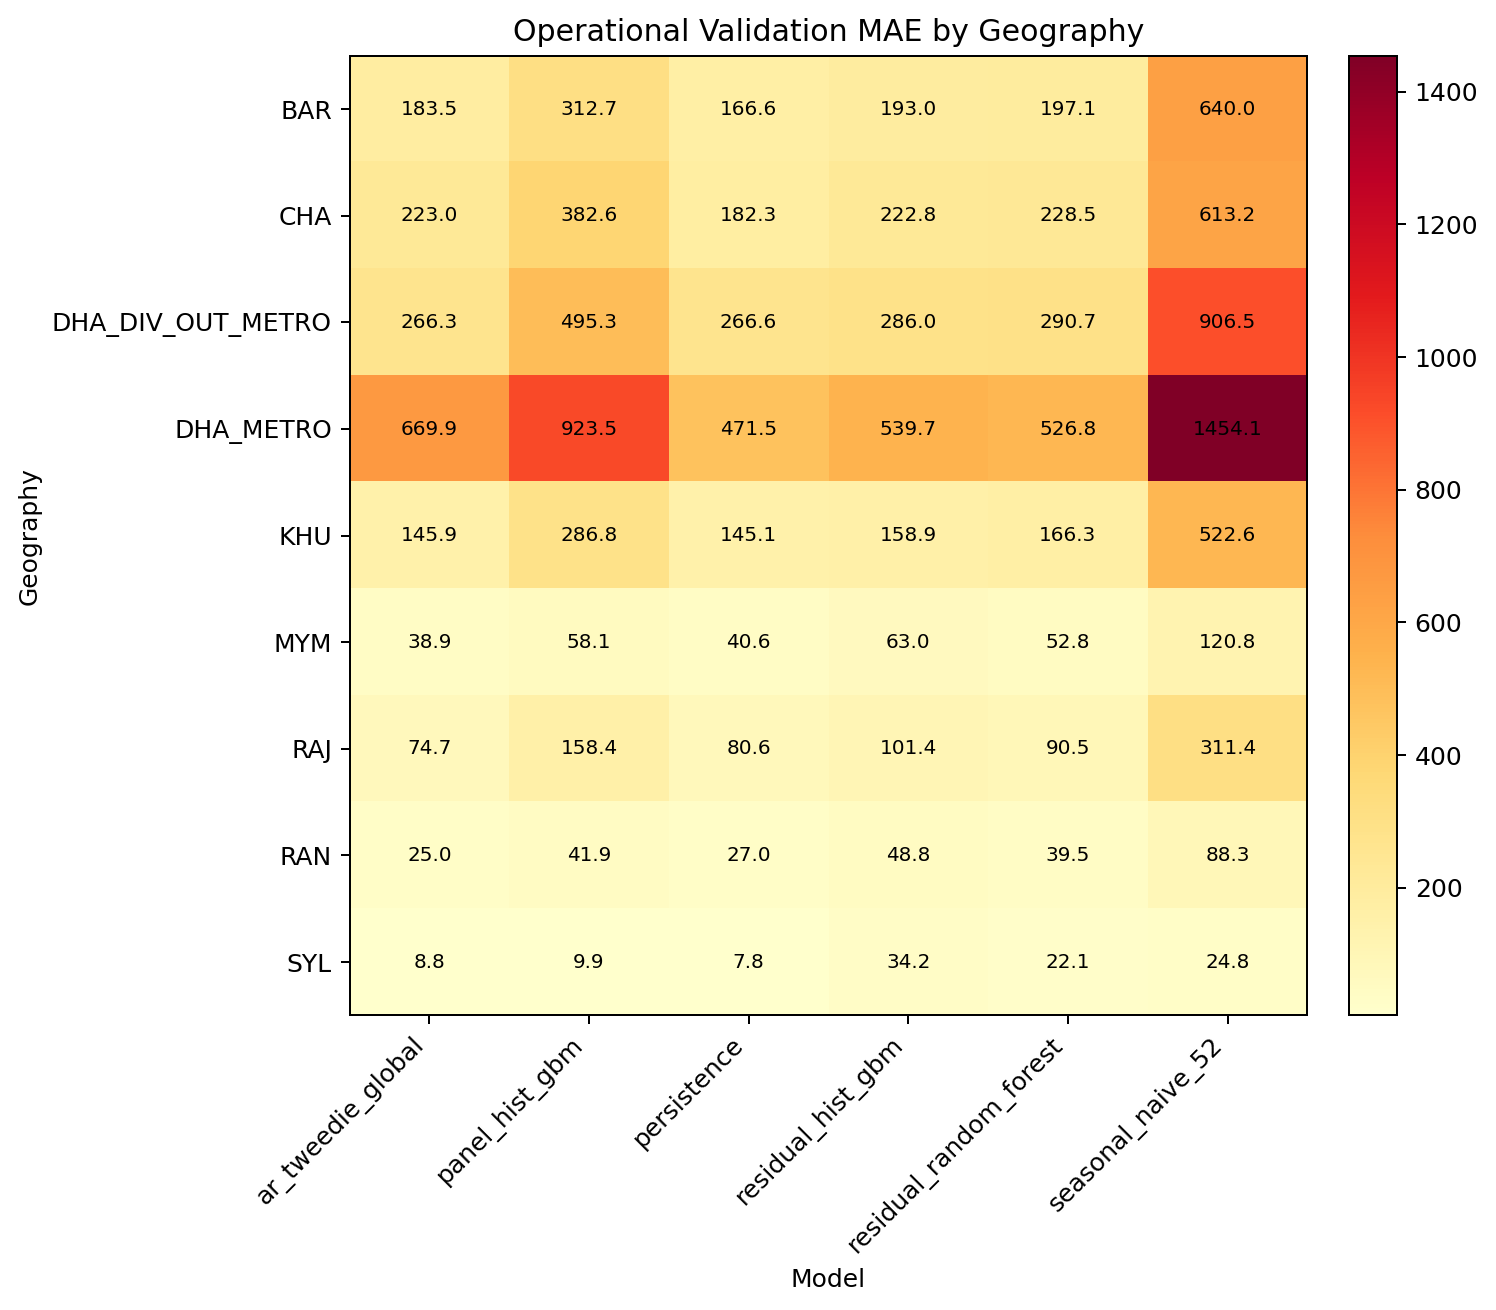
\includegraphics[width=0.78\textwidth]{fig_04_operational_geo_mae_heatmap.png}
\caption{Operational MAE by geography. Scale imbalance is substantial, and some challenger models are more competitive in lower-volume geographies than in Dhaka-dominant series.}
\label{fig:operational-geo}
\end{figure}

\subsection{Experimental Track}
The experimental track extended the horizon to 5--12 weeks and added lagged climate features. Yet persistence again remained the best overall model, with MAE 403.016 and RMSE 510.986. The best experimental challenger was the global histogram gradient boosting model, followed by seasonal naive and the global Tweedie model.

\begin{table}[H]
\centering
\caption{Experimental validation leaderboard.}
\label{tab:experimental-leaderboard}
\begin{tabular}{lrr}
\toprule
Model & MAE & RMSE \\
\midrule
Persistence & 403.016 & 510.986 \\
Panel HistGBM & 516.184 & 692.385 \\
Seasonal naive$_{52}$ & 521.907 & 716.453 \\
AR Tweedie global & 540.113 & 714.009 \\
\bottomrule
\end{tabular}
\end{table}

The experimental result does not imply that climate is irrelevant to dengue. Instead, it shows that the current climate-augmented forecasting setup did not yield an operationally superior predictive system. That may reflect several factors at once: incomplete real-time climate coverage, short sample length, nonstationary outbreak regimes, and the fact that strong recent case history already explains much of the short-to-medium-horizon signal.

\subsection{Training Interpretation and Model Failure Modes}
The model comparisons also exposed distinct failure modes. The free-running global histogram gradient boosting model could be highly competitive in calmer windows but was much less reliable under large regime shifts. The global Tweedie model was comparatively strong in several lower-volume geographies, but occasionally required the operational stability guard. The residual-correction models were more stable than the unconstrained panel GBM and are therefore attractive future candidates, but they still did not beat persistence overall.

This is a useful finding for manuscript interpretation. The main obstacle is not the absence of any predictive structure beyond persistence. Rather, it is the difficulty of converting that extra structure into a model that improves robustly across all the conditions represented in the validation folds.

\subsection{Illustrative Current Forecast}
Because persistence remained the strongest operational model, it was selected as the current primary forecasting rule for the latest available origin week, 2025-09-15. At the country-total level, the persistence forecast was 0.0 for horizons 1--4, reflecting zero observed bottom-level counts at the most recent origin. Challenger models allowed modest rebounds, ranging from 15.0 to 123.2 by horizon 4 for the residual random forest and from 27.1 to 70.2 for the Tweedie model, whereas seasonal naive implied an implausibly large rebound based on the previous year.

\begin{figure}[H]
\centering
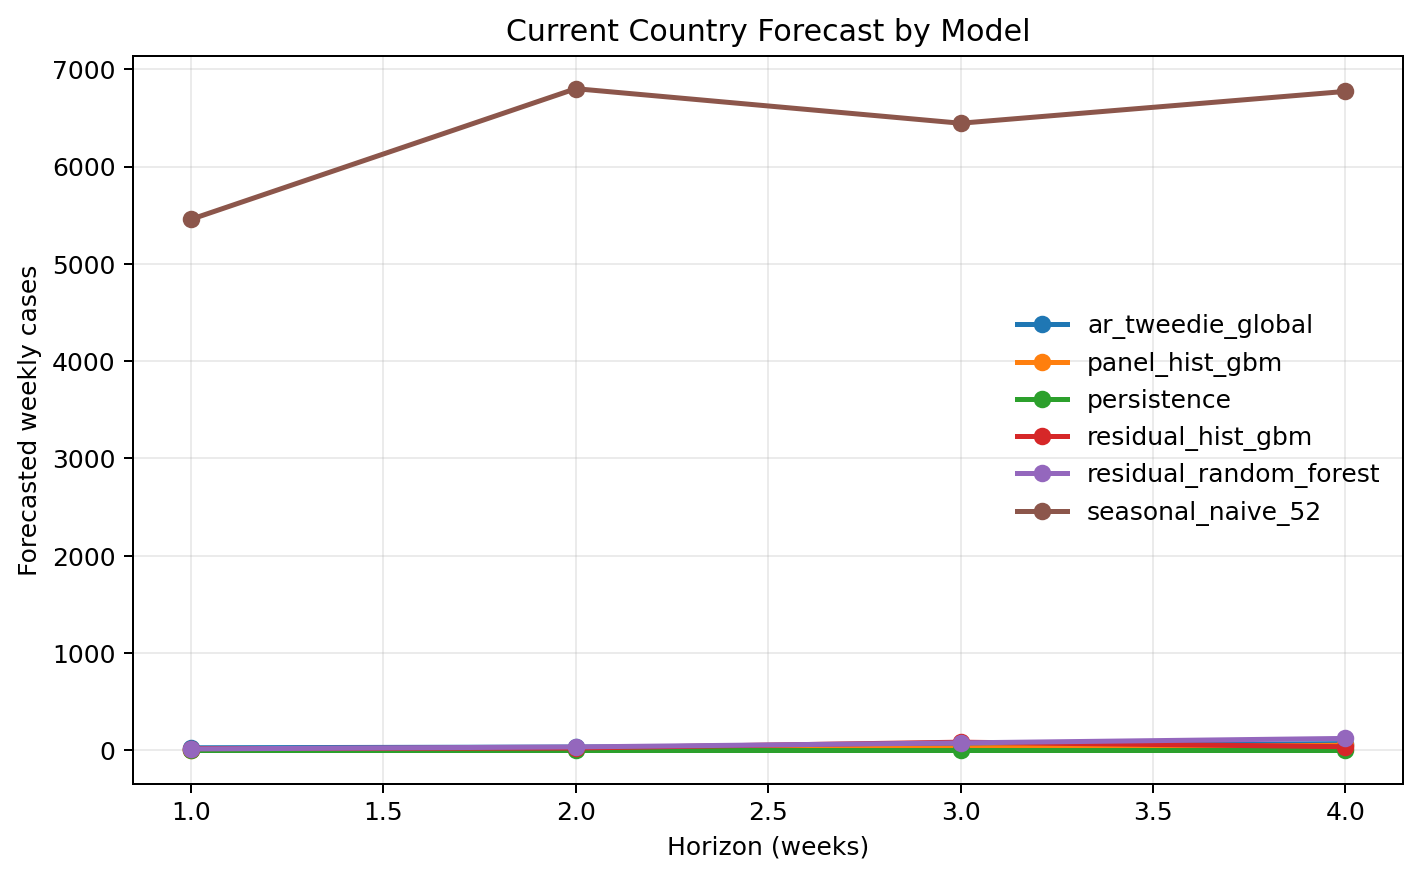
\includegraphics[width=0.82\textwidth]{fig_05_current_country_forecasts.png}
\caption{Illustrative current operational forecast at the latest origin week. The selected primary forecast remains the persistence baseline.}
\label{fig:current-forecast}
\end{figure}

\section{Discussion}
This study was designed to answer a practical forecasting question under real operational constraints, and the main result is straightforward: persistence remains the strongest short-horizon weekly dengue forecasting model overall in the current Bangladesh panel. That is not a trivial result. In a field where more complex models are often assumed to be inherently better, this study shows that once hierarchy consistency, rolling-origin validation, geography-level scoring, and real-time covariate availability are taken seriously, the best model may still be the strongest simple baseline.

The result is scientifically important for three reasons. First, it shows that the dominant predictive signal in the current data is short-run autoregressive momentum, not long-memory annual repetition. Second, it demonstrates that plausible climate associations do not automatically translate into operational forecasting gains when the covariate stream is incomplete at the most recent dates. Third, it suggests that the most promising model-development path is not unrestricted complexity, but persistence-anchored residual learning that preserves the strongest baseline while modeling controlled deviations from it.

The fold- and geography-level analyses sharpen that interpretation. Several challengers were genuinely competitive. The global histogram gradient boosting model won multiple folds. The residual histogram gradient boosting model performed best during the major outbreak fold. The Tweedie model was strongest in several lower-volume geographies. These are not signs of model irrelevance. They are signs that the underlying signal is heterogeneous and regime-dependent, and that the missing ingredient is robustness rather than raw flexibility.

For a public health manuscript, the operational implication is clear. If a model is to be used for short-horizon dengue preparedness in Bangladesh today, it should not require fresh weather data that are not consistently available, and it should not be promoted merely because it wins in a single fold or on pooled national totals. It should beat persistence repeatedly, across lead times and across both Dhaka-dominant and sparse peripheral geographies. At present, no challenger meets that standard.

\section{Limitations}
This study has several limitations. First, the available time series remain short for modern multi-series forecasting, with only 195 weekly observations per geography. Second, a few large outbreak windows contribute disproportionately to the signal, making generalization challenging. Third, climate covariates ended 11 weeks before the latest case week, limiting their operational usefulness despite plausible lead-lag relationships. Fourth, the current study focused on point forecasting; interval prediction and calibrated probabilistic forecasts remain future work. Finally, although rolling-origin backtesting is far more realistic than a single random split, the study is still limited to one national surveillance system and has not yet undergone external validation in a separate country or institutional deployment setting.

\section{Conclusion}
We reframed dengue forecasting in Bangladesh as a hierarchy-aware, weekly, multi-geography count forecasting problem and evaluated a transparent model ladder using rolling-origin backtesting. The clearest result is that persistence remains the strongest operational 1--4 week model overall. More flexible challengers, especially persistence-anchored residual models and pooled count models, show localized promise but do not yet deliver stable enough gains for operational promotion. The practical next step is therefore not simply to add more model capacity. It is to improve data timeliness, build regime-aware residual features, perform deeper geography-level error analysis, and then retest whether any challenger can beat persistence under the same rigorous evaluation design.

\section*{Data Availability}
The processed datasets, artifact bundles, figures, and manuscript assets used in this study are archived in the project repository. Access to upstream raw surveillance and environmental sources should remain subject to the original data providers' access terms and reporting policies.

\section*{Code Availability}
All code used to construct the hierarchy-fixed panel, run exploratory diagnostics, execute rolling-origin backtests, generate operational forecasts, and build manuscript figures and tables is available in the accompanying project repository.

\section*{Competing Interests}
The authors declare that they have no competing interests.

\section*{Funding}
Funding information to be added.

\section*{Acknowledgements}
Acknowledgements to be added.

% Journal-porting notes:
% 1. Once a target journal is selected, migrate this source into the journal's LaTeX template.
% 2. Add venue-specific abstract structure, author blocks, data/code statements, and reference style.
% 3. Consider moving the illustrative current forecast subsection to the Supplement if the target venue prefers a leaner main text.

\bibliographystyle{unsrtnat}
\bibliography{references}

\end{document}
